\section{Vision-Based Robotic Grasping of Diverse Objects}

\begin{frame}{Vision-Based Robotic Grasping of Diverse Objects}{Objective}
    \centering
    \begin{columns}%
        \begin{column}{0.5\textwidth}%
            \centering
            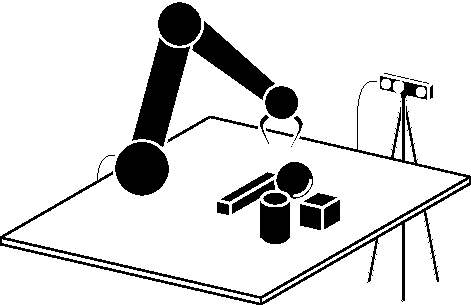
\includegraphics[height=4.3cm]{graphics/setup_sketch.pdf}
        \end{column}
        %
        \begin{column}{0.5\textwidth}%
            \centering
            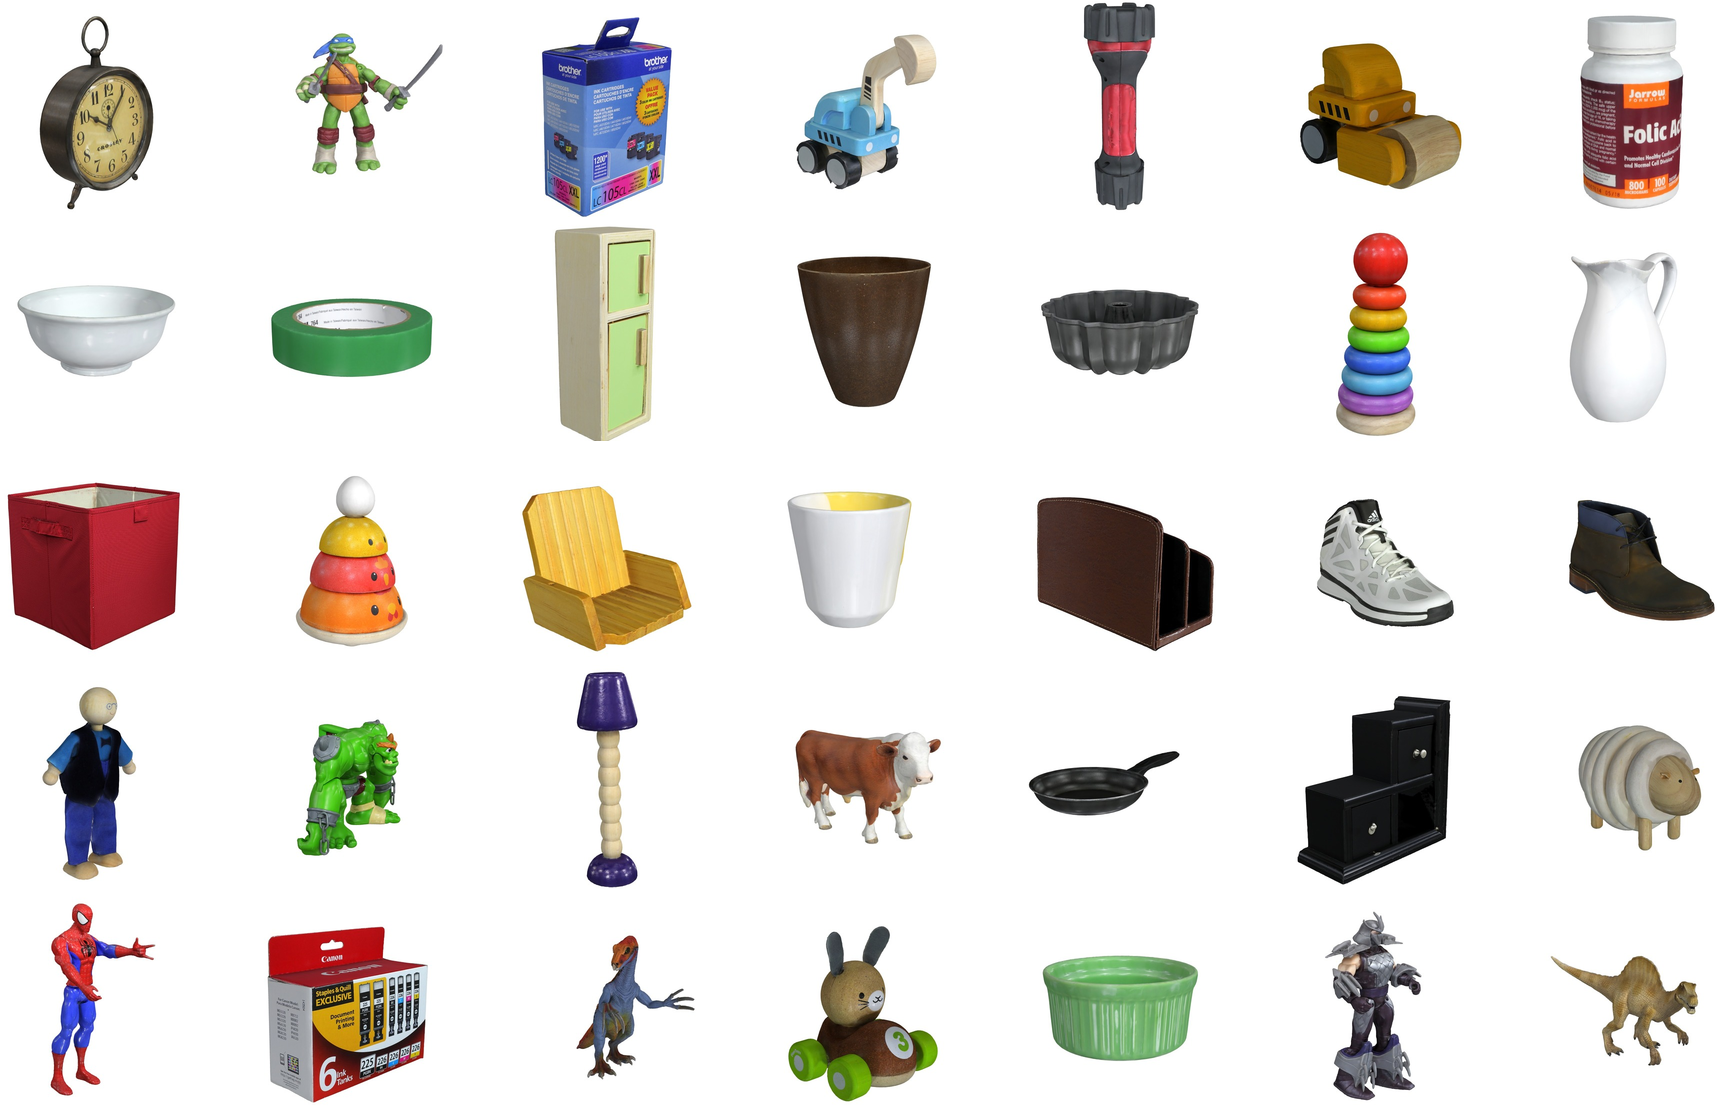
\includegraphics[height=4.3cm]{graphics/training_set.png}
        \end{column}
    \end{columns}
\end{frame}

\begin{frame}{Vision-Based Robotic Grasping of Diverse Objects}{Approach}
    \centering
    {\Large Reinforcement Learning}

    \vspace{0.25cm}

    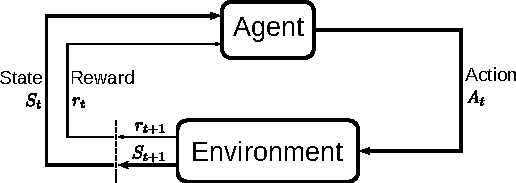
\includegraphics[width=0.75\textwidth]{graphics/mdp_loop.pdf}
\end{frame}

\begin{frame}{Vision-Based Robotic Grasping of Diverse Objects}{End-to-End Policy}
    \centering
    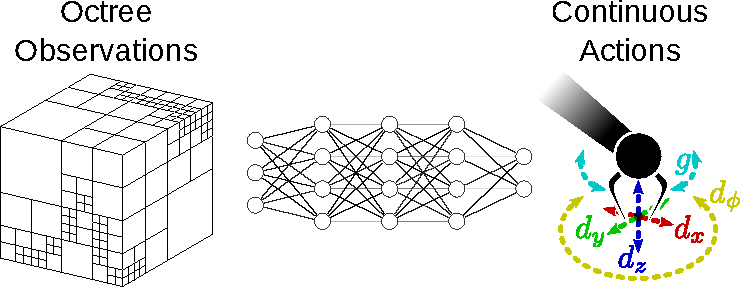
\includegraphics[width=0.85\textwidth]{graphics/end_to_end_policy.pdf}
\end{frame}

\begin{frame}{Vision-Based Robotic Grasping of Diverse Objects}{Sim2Real Transfer}
    \centering
    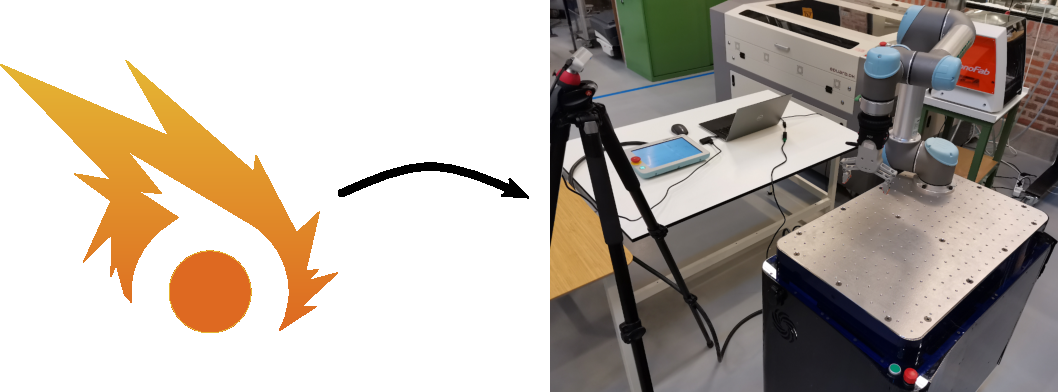
\includegraphics[width=0.95\textwidth]{graphics/sim2real.pdf}
\end{frame}


\section{Gym-Ignition}

\begin{frame}{How to Create RL Environments inside Ignition Gazebo?}{Gym-Ignition}
    \begin{columns}%
        \begin{column}{0.5\textwidth}%
            \begin{block}{\href{https://github.com/robotology/gym-ignition}{Gym-Ignition}}
                \begin{itemize}
                    \item Interface for Ignition Gazebo
                    \item Tooling for creation of OpenAI Gym environments%
                          \begin{itemize}
                              \item Compatibility with RL frameworks (e.g.~\href{https://github.com/DLR-RM/stable-baselines3}{Stable Baselines3})
                          \end{itemize}
                \end{itemize}
            \end{block}
        \end{column}
        %
        \begin{column}{0.5\textwidth}%
            \centering
            \href{https://github.com/robotology/gym-ignition}{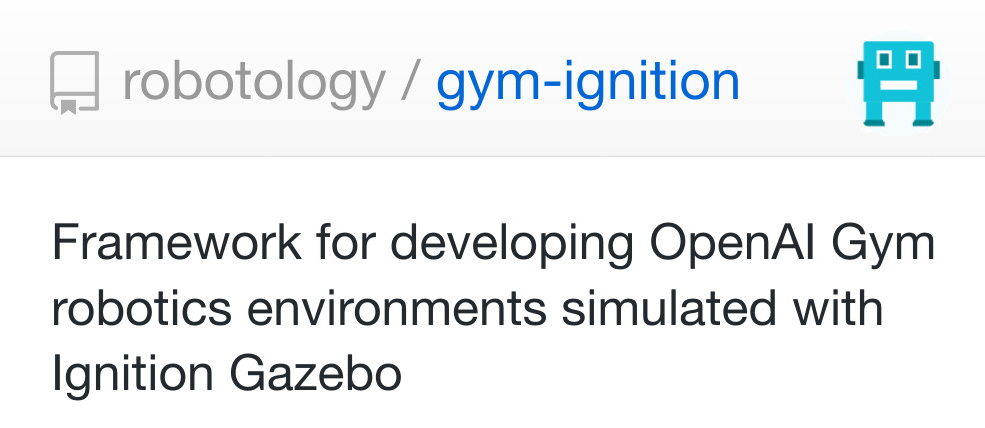
\includegraphics[width=1.0\textwidth]{graphics/gym_ignition.png}}
        \end{column}
    \end{columns}
    \footnoteref{Ferigo et al. 2020. Gym-Ignition: Reproducible Robotic Simulations for Reinforcement Learning. In 2020 IEEE/SICE International Symposium on System Integration (SII). 885–890.}
\end{frame}


\section{Ignition Fuel}

\begin{frame}{Where to Find Models?}{Ignition Fuel}
    \centering
    \begin{columns}%
        \begin{column}{0.69\textwidth}%
            \centering
            \href{https://app.ignitionrobotics.org/GoogleResearch/fuel/collections/Google Scanned Objects}{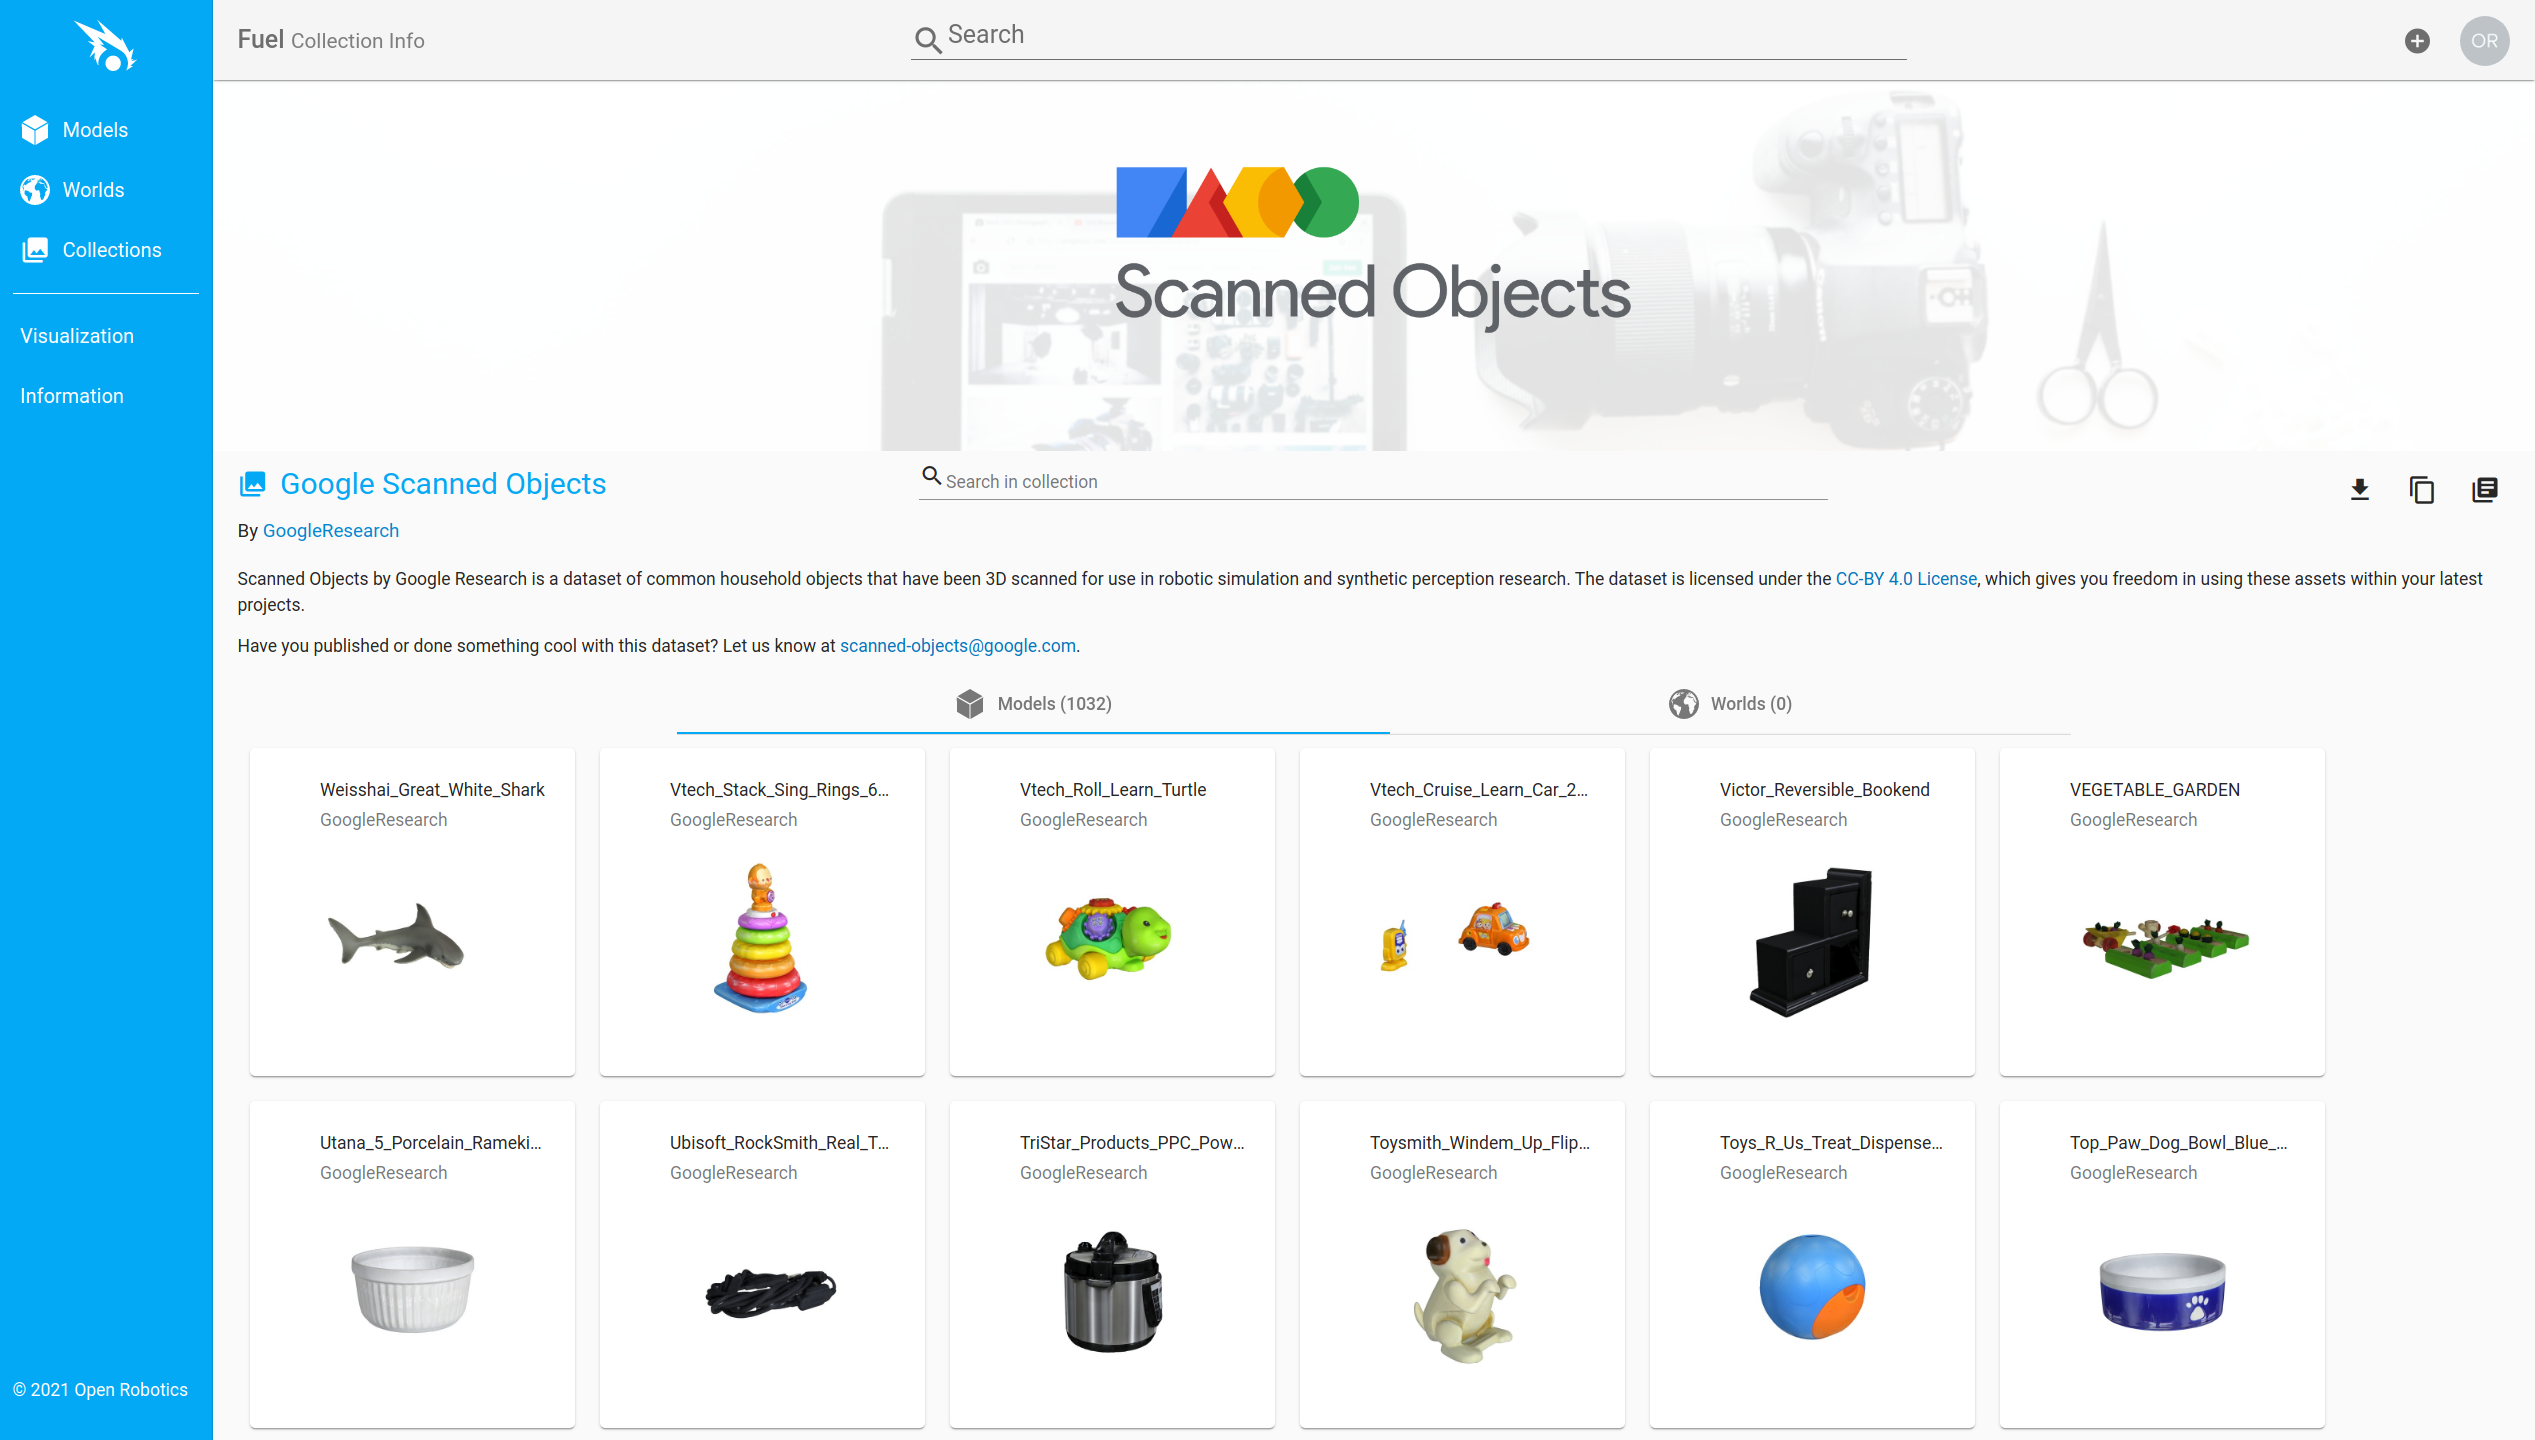
\includegraphics[width=\textwidth]{graphics/fuel_google_scanned_objects.png}}
        \end{column}
        %
        \begin{column}{0.31\textwidth}%
            \centering
            \begin{block}{No Inertial Properties?}
                \begin{itemize}
                    \item Estimate
                \end{itemize}
            \end{block}
            \begin{block}{Too Much Geometry?}
                \begin{itemize}
                    \item Decimate
                \end{itemize}
            \end{block}
            \begin{block}{Open-Source Libraries}
                \begin{itemize}
                    \item \href{https://github.com/intel-isl/Open3D}{intel-isl/\textbf{Open3D}}
                    \item \href{https://github.com/mikedh/trimesh}{mikedh/\textbf{trimesh}}
                    \item ...
                \end{itemize}
            \end{block}
        \end{column}
    \end{columns}
\end{frame}

\begin{frame}{Models}{Object Datasets (Training | Testing)}
    \centering
    \includegraphics[height=6.5cm]{graphics/datasets_full.png}
\end{frame}

\begin{frame}{Models}{Robots}
    \centering
    \includegraphics[height=6.5cm]{graphics/datasets_full_with_robots.png}
\end{frame}


\section{Domain Randomization}

\begin{frame}{Domain Randomization}{Visual Examples}
    \centering
    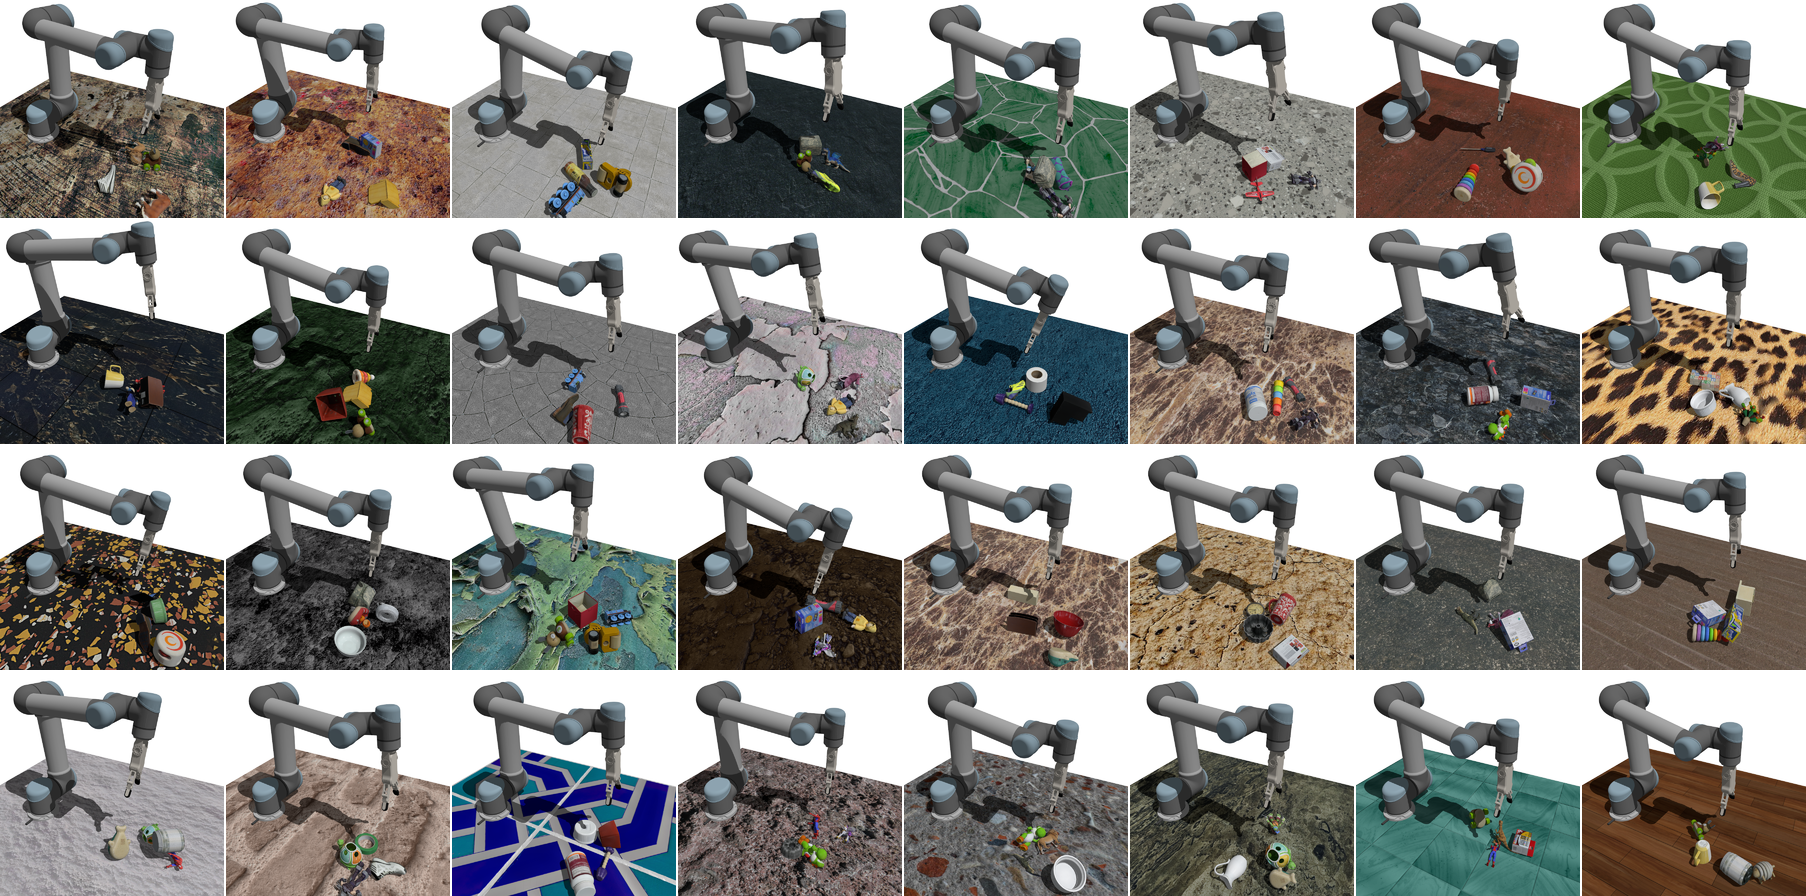
\includegraphics[height=6.5cm]{graphics/domain_randomisation.png}
\end{frame}

\begin{frame}{Domain Randomization}{Further Randomization}
    \begin{columns}%
        \begin{column}{0.35\textwidth}%
            \begin{block}{Random}
                \begin{itemize}
                    \item Objects
                          \begin{itemize}
                              \item Model
                              \item Scale
                              \item Mass
                              \item Friction
                              \item Pose
                          \end{itemize}
                    \item Ground plane texture
                    \item Initial robot configuration
                    \item Camera
                          \begin{itemize}
                              \item Pose
                              \item Sensory noise
                          \end{itemize}
                \end{itemize}
            \end{block}
        \end{column}
        %
        \begin{column}{0.65\textwidth}%
            \centering
            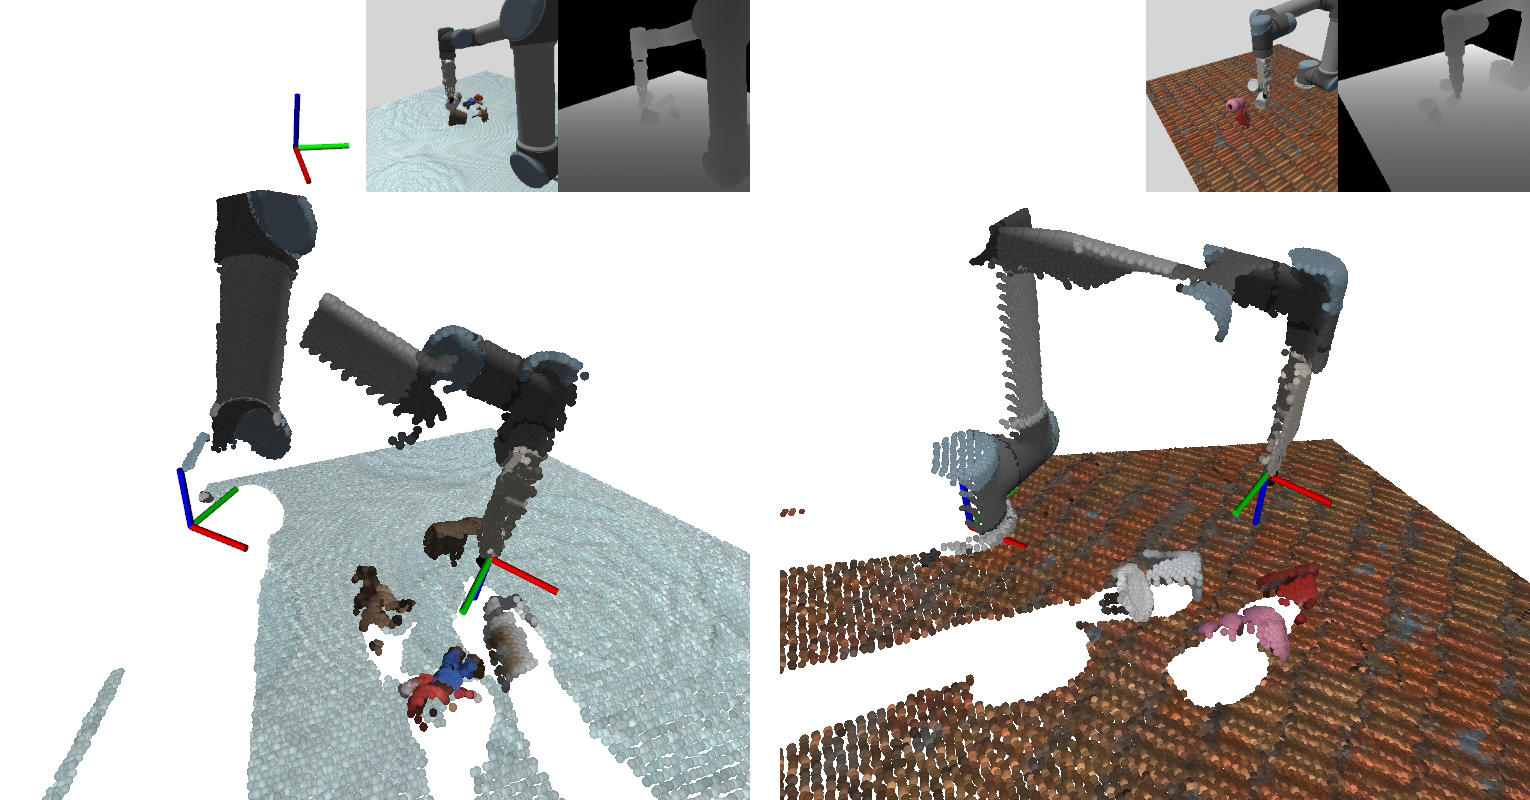
\includegraphics[height=4.75cm]{graphics/random_camera_pose.png}
        \end{column}
    \end{columns}
\end{frame}


\section{Training}

% \begin{frame}{Training of New Agents}{Simulation - Panda (Video Example)}
%     \centering
%     \vspace{-0.4cm}
%     \scalebox{0.25}{%
%         \def \vidwidth{1500px}%
%         \def \vidheight{800px}%
%         \href{https://www.youtube.com/watch?v=1-cudiW4eaU&t=0s}{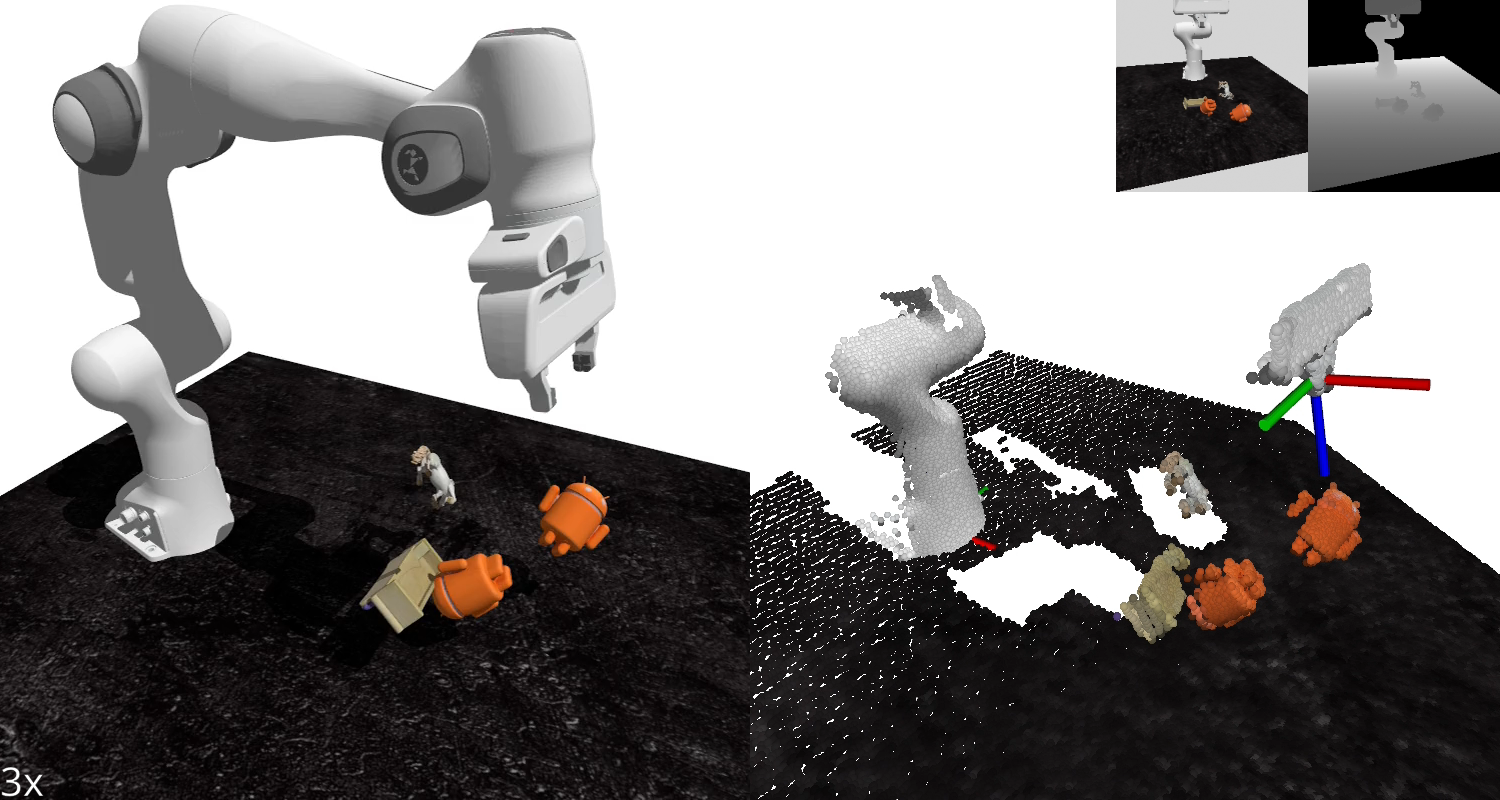
\includegraphics[width=\vidwidth,height=\vidheight]{videos/sim_panda_0.png}}
%     }
% \end{frame}

\begin{frame}{Training}{Simulation - Panda (Video Example)}
    \centering
    \scalebox{0.13}{%
        \def \vidwidth{1000px}%
        \def \vidheight{900px}%
        \includemedia[width=\vidwidth,height=\vidheight,activate=pageopen,
            passcontext,
            transparent,
            keepaspectratio,
            final,
            noplaybutton,
            addresource=videos/training_0.mp4,
            flashvars={source=videos/training_0.mp4 &loop=true}
        ]{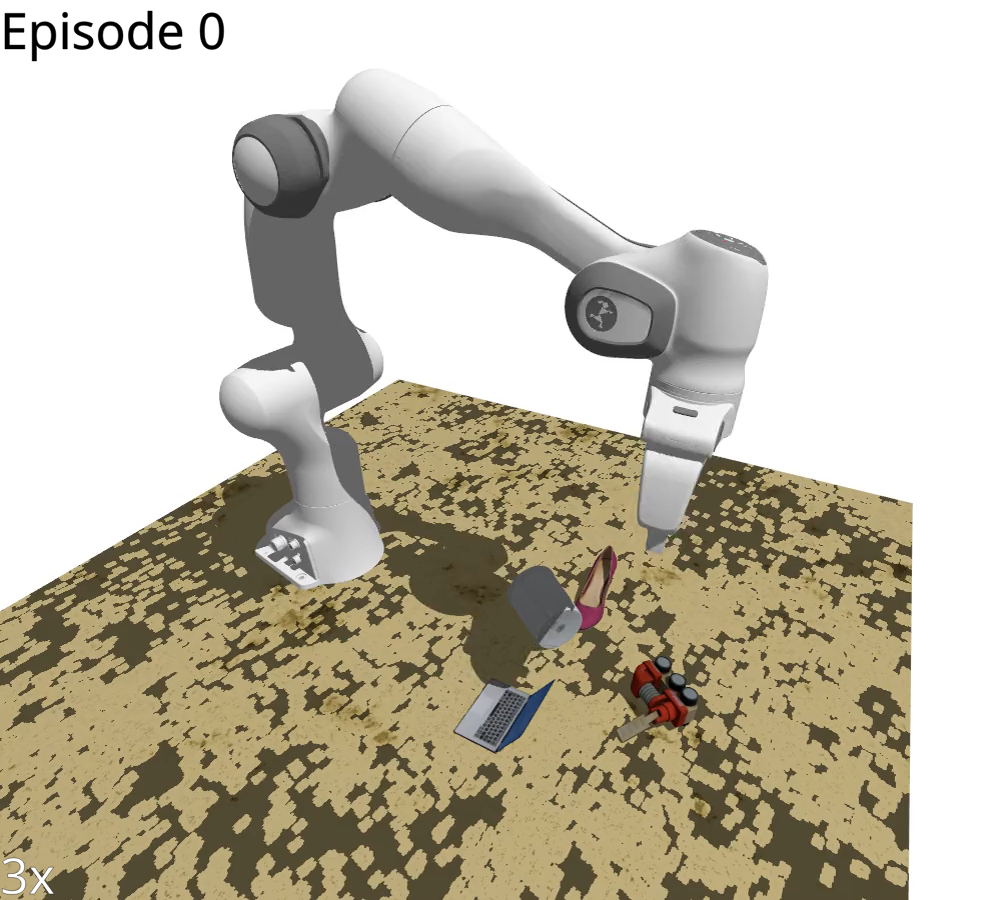
\includegraphics[width=\vidwidth,height=\vidheight]{videos/training_0_0.png}}{VPlayer.swf}
    }%
    \scalebox{0.13}{%
        \def \vidwidth{1000px}%
        \def \vidheight{900px}%
        \includemedia[width=\vidwidth,height=\vidheight,activate=pageopen,
            passcontext,
            transparent,
            keepaspectratio,
            final,
            noplaybutton,
            addresource=videos/training_100.mp4,
            flashvars={source=videos/training_100.mp4 &loop=true}
        ]{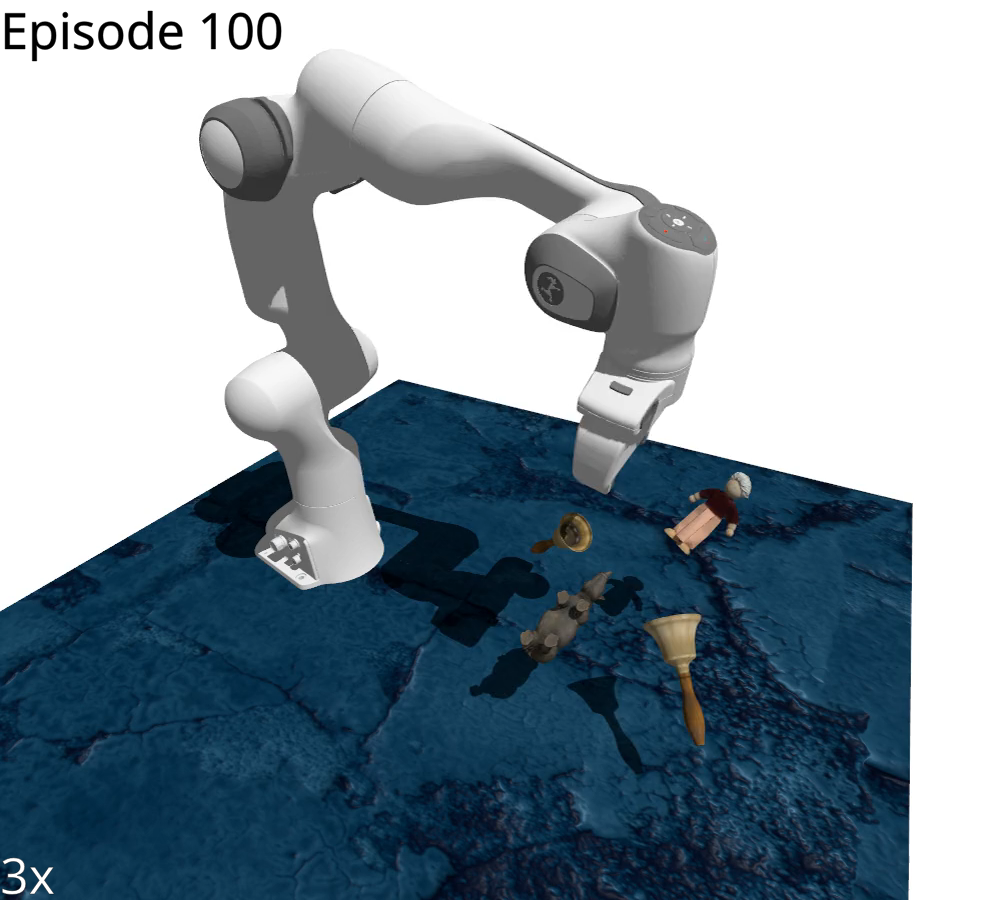
\includegraphics[width=\vidwidth,height=\vidheight]{videos/training_100_0.png}}{VPlayer.swf}
    }%
    \scalebox{0.13}{%
        \def \vidwidth{1000px}%
        \def \vidheight{900px}%
        \includemedia[width=\vidwidth,height=\vidheight,activate=pageopen,
            passcontext,
            transparent,
            keepaspectratio,
            final,
            noplaybutton,
            addresource=videos/training_1000.mp4,
            flashvars={source=videos/training_1000.mp4 &loop=true}
        ]{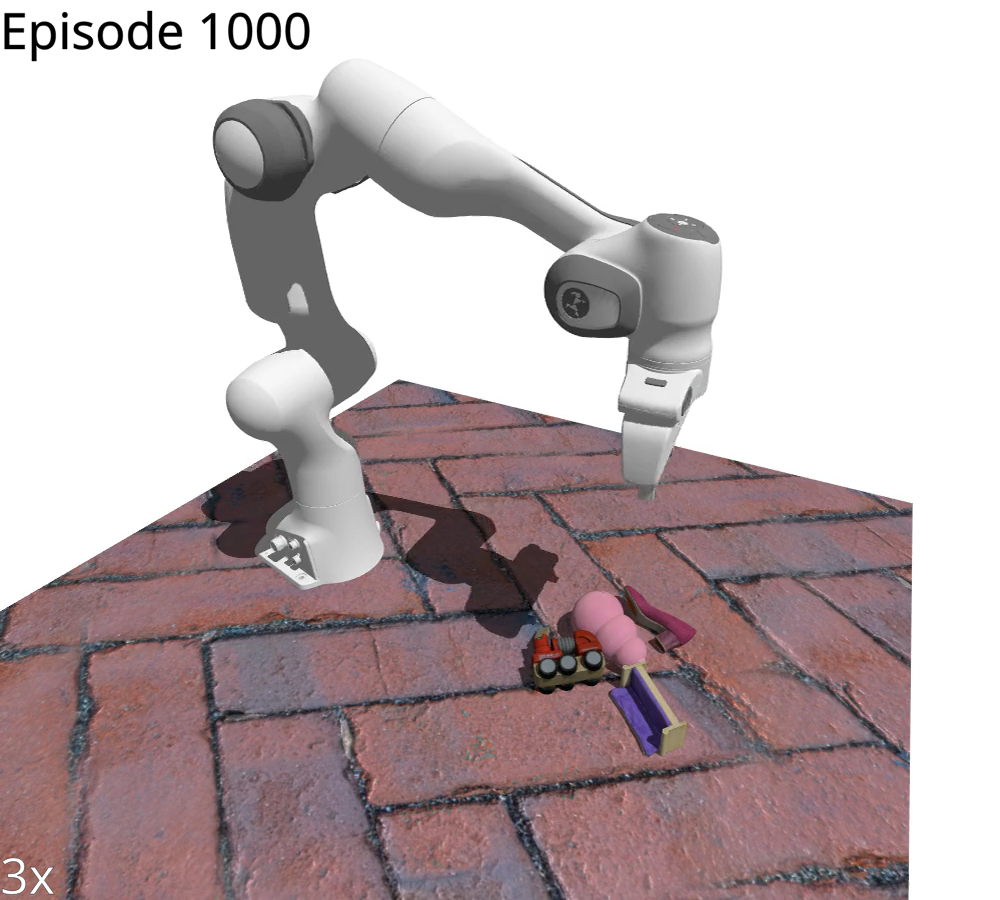
\includegraphics[width=\vidwidth,height=\vidheight]{videos/training_1000_0.png}}{VPlayer.swf}
    }
\end{frame}


\section{Trained Agents}

\begin{frame}{Trained Agent}{Simulation - Panda (Video Example)}
    \centering
    \vspace{-0.4cm}
    \scalebox{0.25}{%
        \def \vidwidth{1500px}%
        \def \vidheight{800px}%
        \includemedia[width=\vidwidth,height=\vidheight,activate=pageopen,
            passcontext,
            transparent,
            keepaspectratio,
            final,
            noplaybutton,
            addresource=videos/sim_panda.mp4,
            flashvars={source=videos/sim_panda.mp4 &loop=true}
        ]{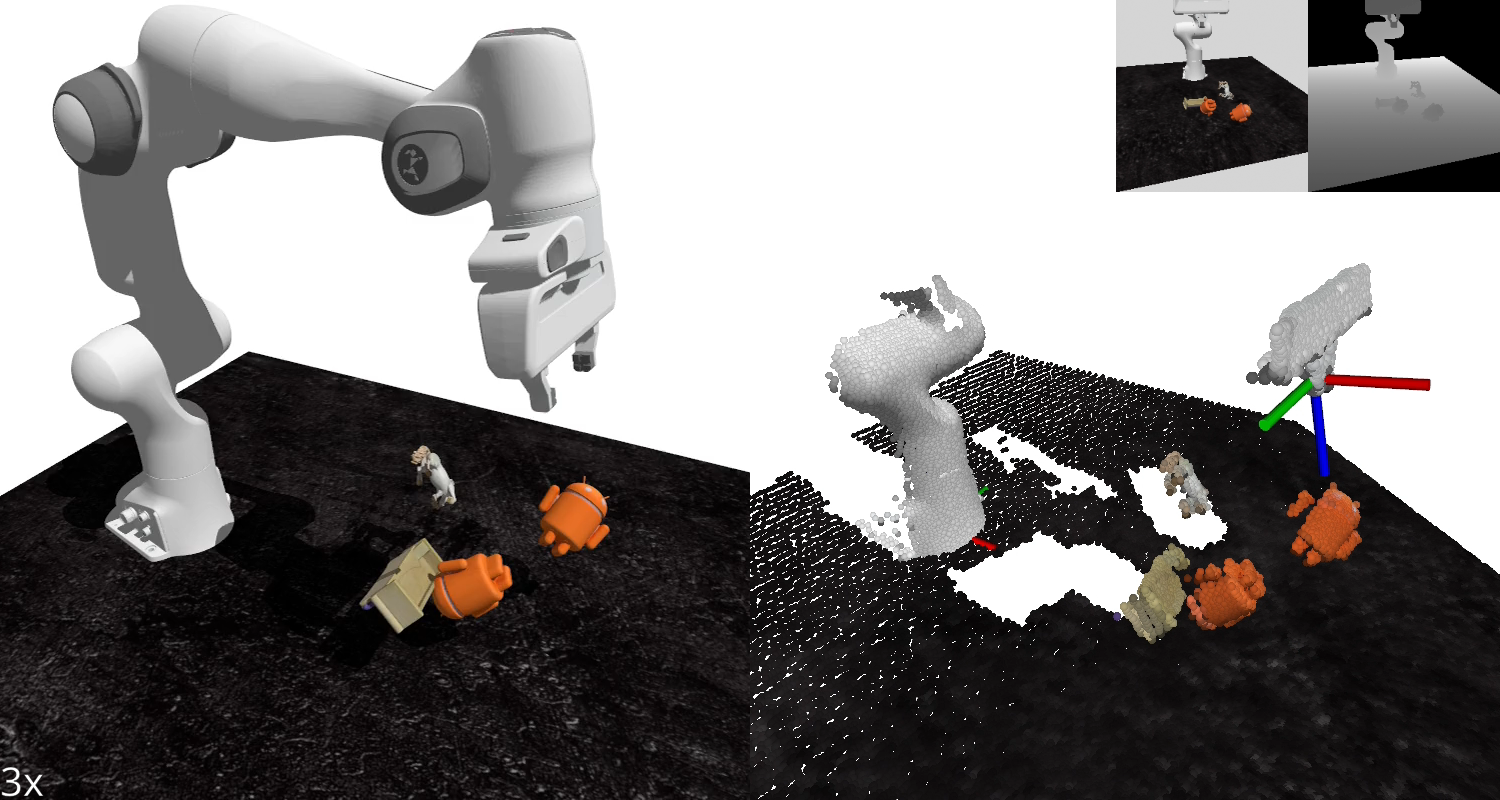
\includegraphics[width=\vidwidth,height=\vidheight]{videos/sim_panda_0.png}}{VPlayer.swf}
    }
\end{frame}

\begin{frame}{Trained Agent}{Simulation - UR 5 (Video Example)}
    \centering
    \vspace{-0.4cm}
    \scalebox{0.25}{%
        \def \vidwidth{1500px}%
        \def \vidheight{800px}%
        \includemedia[width=\vidwidth,height=\vidheight,activate=pageopen,
            passcontext,
            transparent,
            keepaspectratio,
            final,
            noplaybutton,
            addresource=videos/sim_ur5_rg2.mp4,
            flashvars={source=videos/sim_ur5_rg2.mp4 &loop=true}
        ]{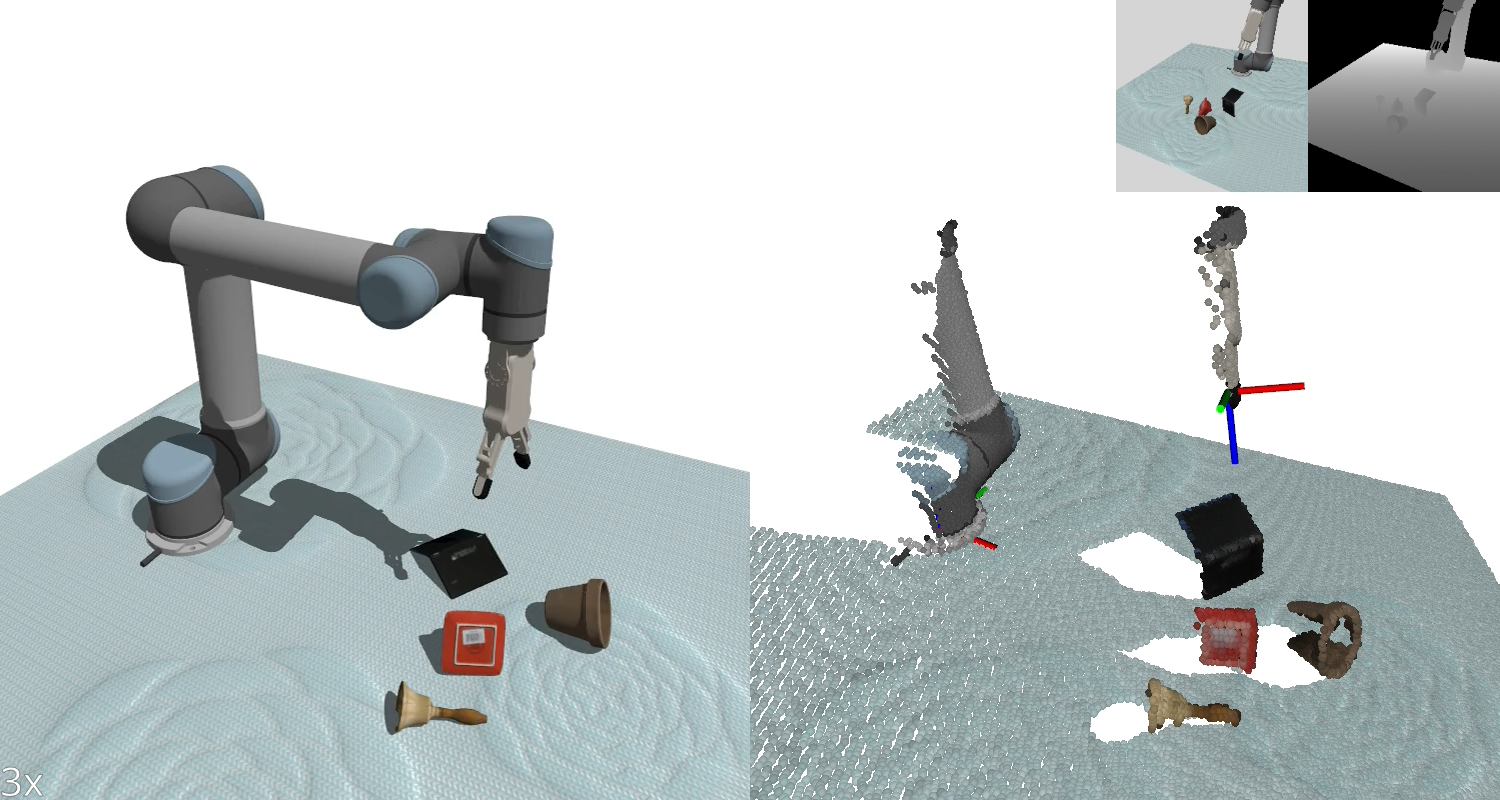
\includegraphics[width=\vidwidth,height=\vidheight]{videos/sim_ur5_rg2_0.png}}{VPlayer.swf}
    }
\end{frame}


\section{Sim2Real}

\begin{frame}{Sim2Real}{Real - UR 5 (Video Example)}
    \centering
    \scalebox{0.175}{%
        \def \vidwidth{2240px}%
        \def \vidheight{1000px}%
        \includemedia[width=\vidwidth,height=\vidheight,activate=pageopen,
            passcontext,
            transparent,
            keepaspectratio,
            final,
            noplaybutton,
            addresource=videos/sim2real.mp4,
            flashvars={source=videos/sim2real.mp4 &loop=true}
        ]{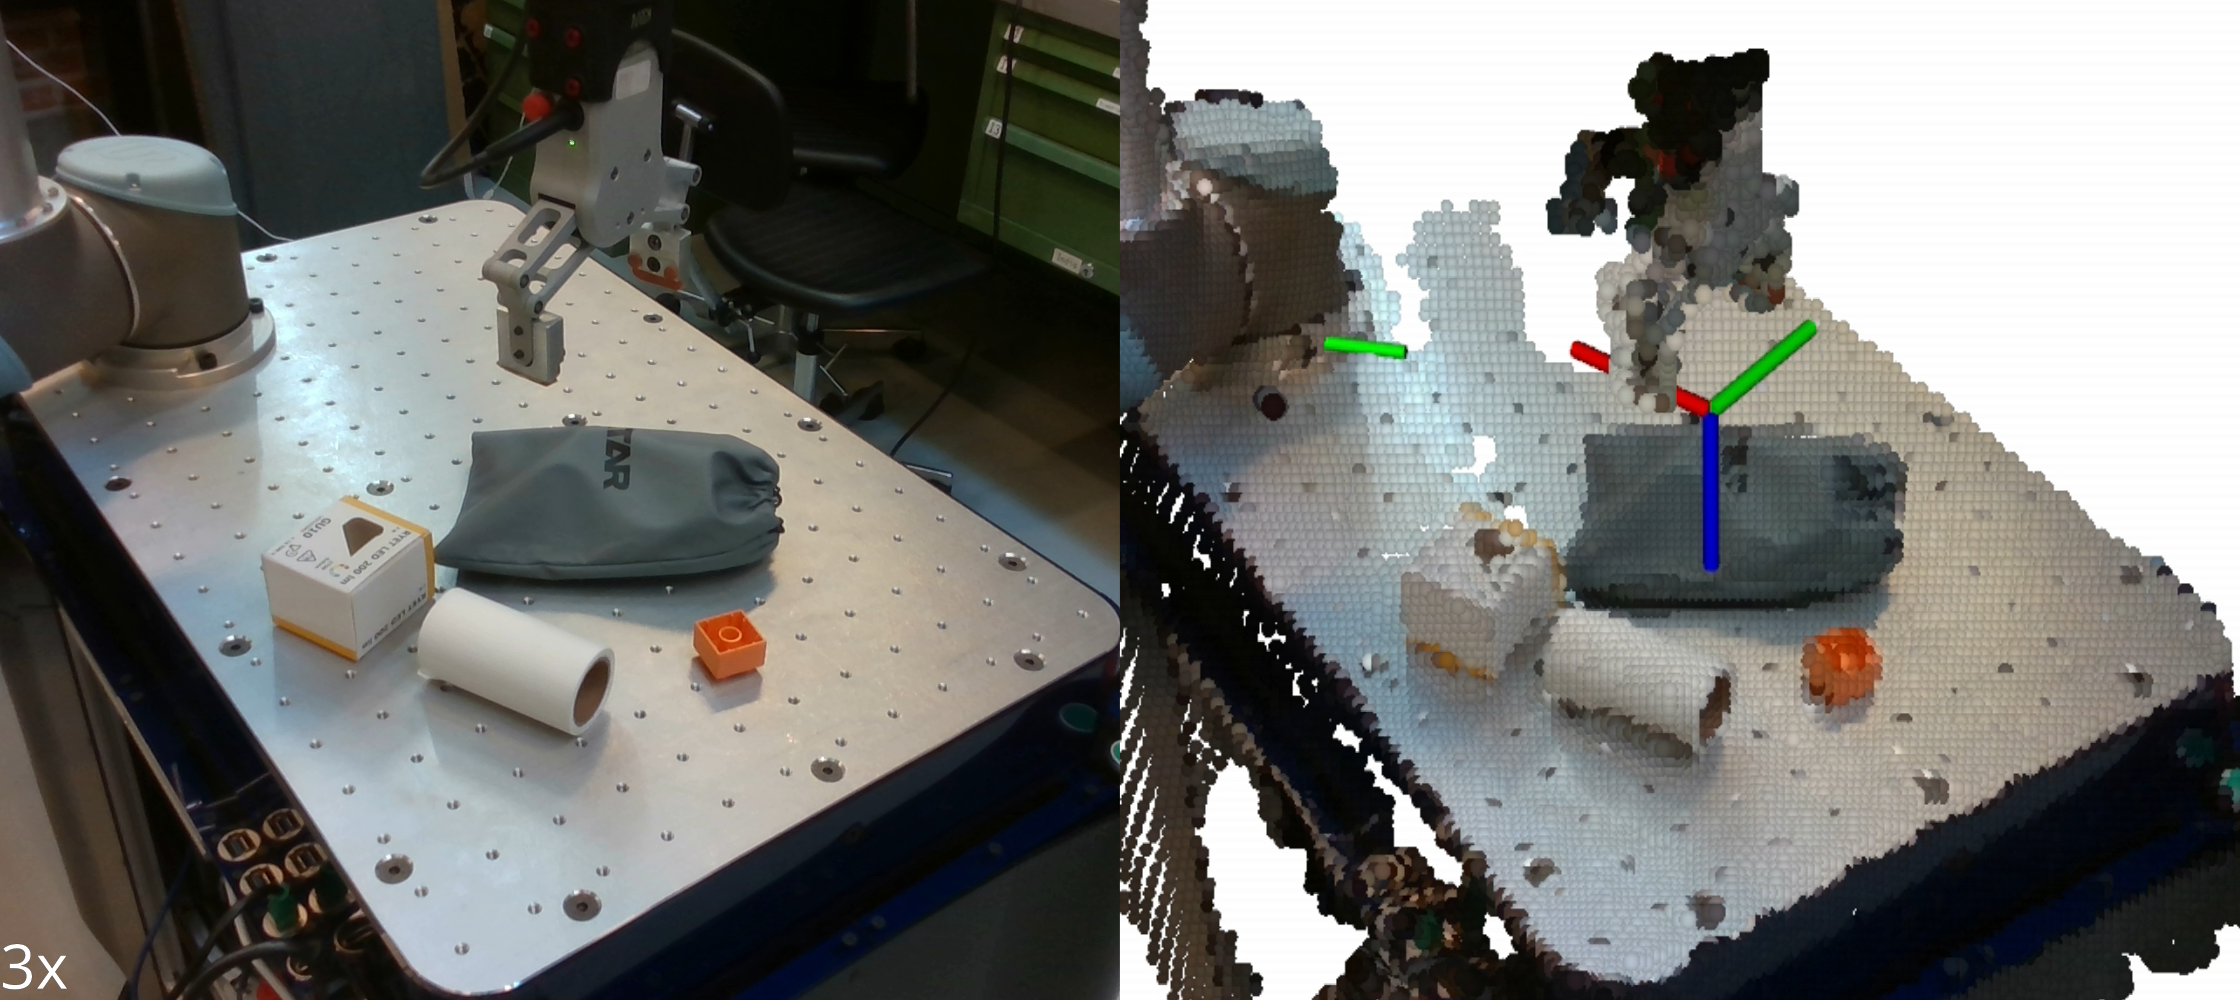
\includegraphics[width=\vidwidth,height=\vidheight]{videos/sim2real_0.png}}{VPlayer.swf}
    }
\end{frame}


\section{GitHub Repository and Examples}

\begin{frame}[fragile]{GitHub Repository and Examples}{\href{https://github.com/AndrejOrsula/drl_grasping}{AndrejOrsula/\textbf{drl\_grasping}}}
    \vspace{-0.3cm}

    \begin{columns}%
        \begin{column}{0.325\textwidth}%
            \begin{block}{\href{https://hub.docker.com/repository/docker/andrejorsula/drl_grasping}{Pre-Built Docker Image}}
                {\scriptsize%
                    \begin{itemize}
                        \item \textasciitilde7.5 GB
                    \end{itemize}
                }%
                \begin{lstlisting}[language=bash,basicstyle=\tiny,stepnumber=1,numbersep=10pt,tabsize=4,showspaces=false,showstringspaces=false]
        docker pull andrejorsula/drl_grasping:latest
                \end{lstlisting}
            \end{block}
        \end{column}
        %
        \begin{column}{0.6\textwidth}%
            \centering
            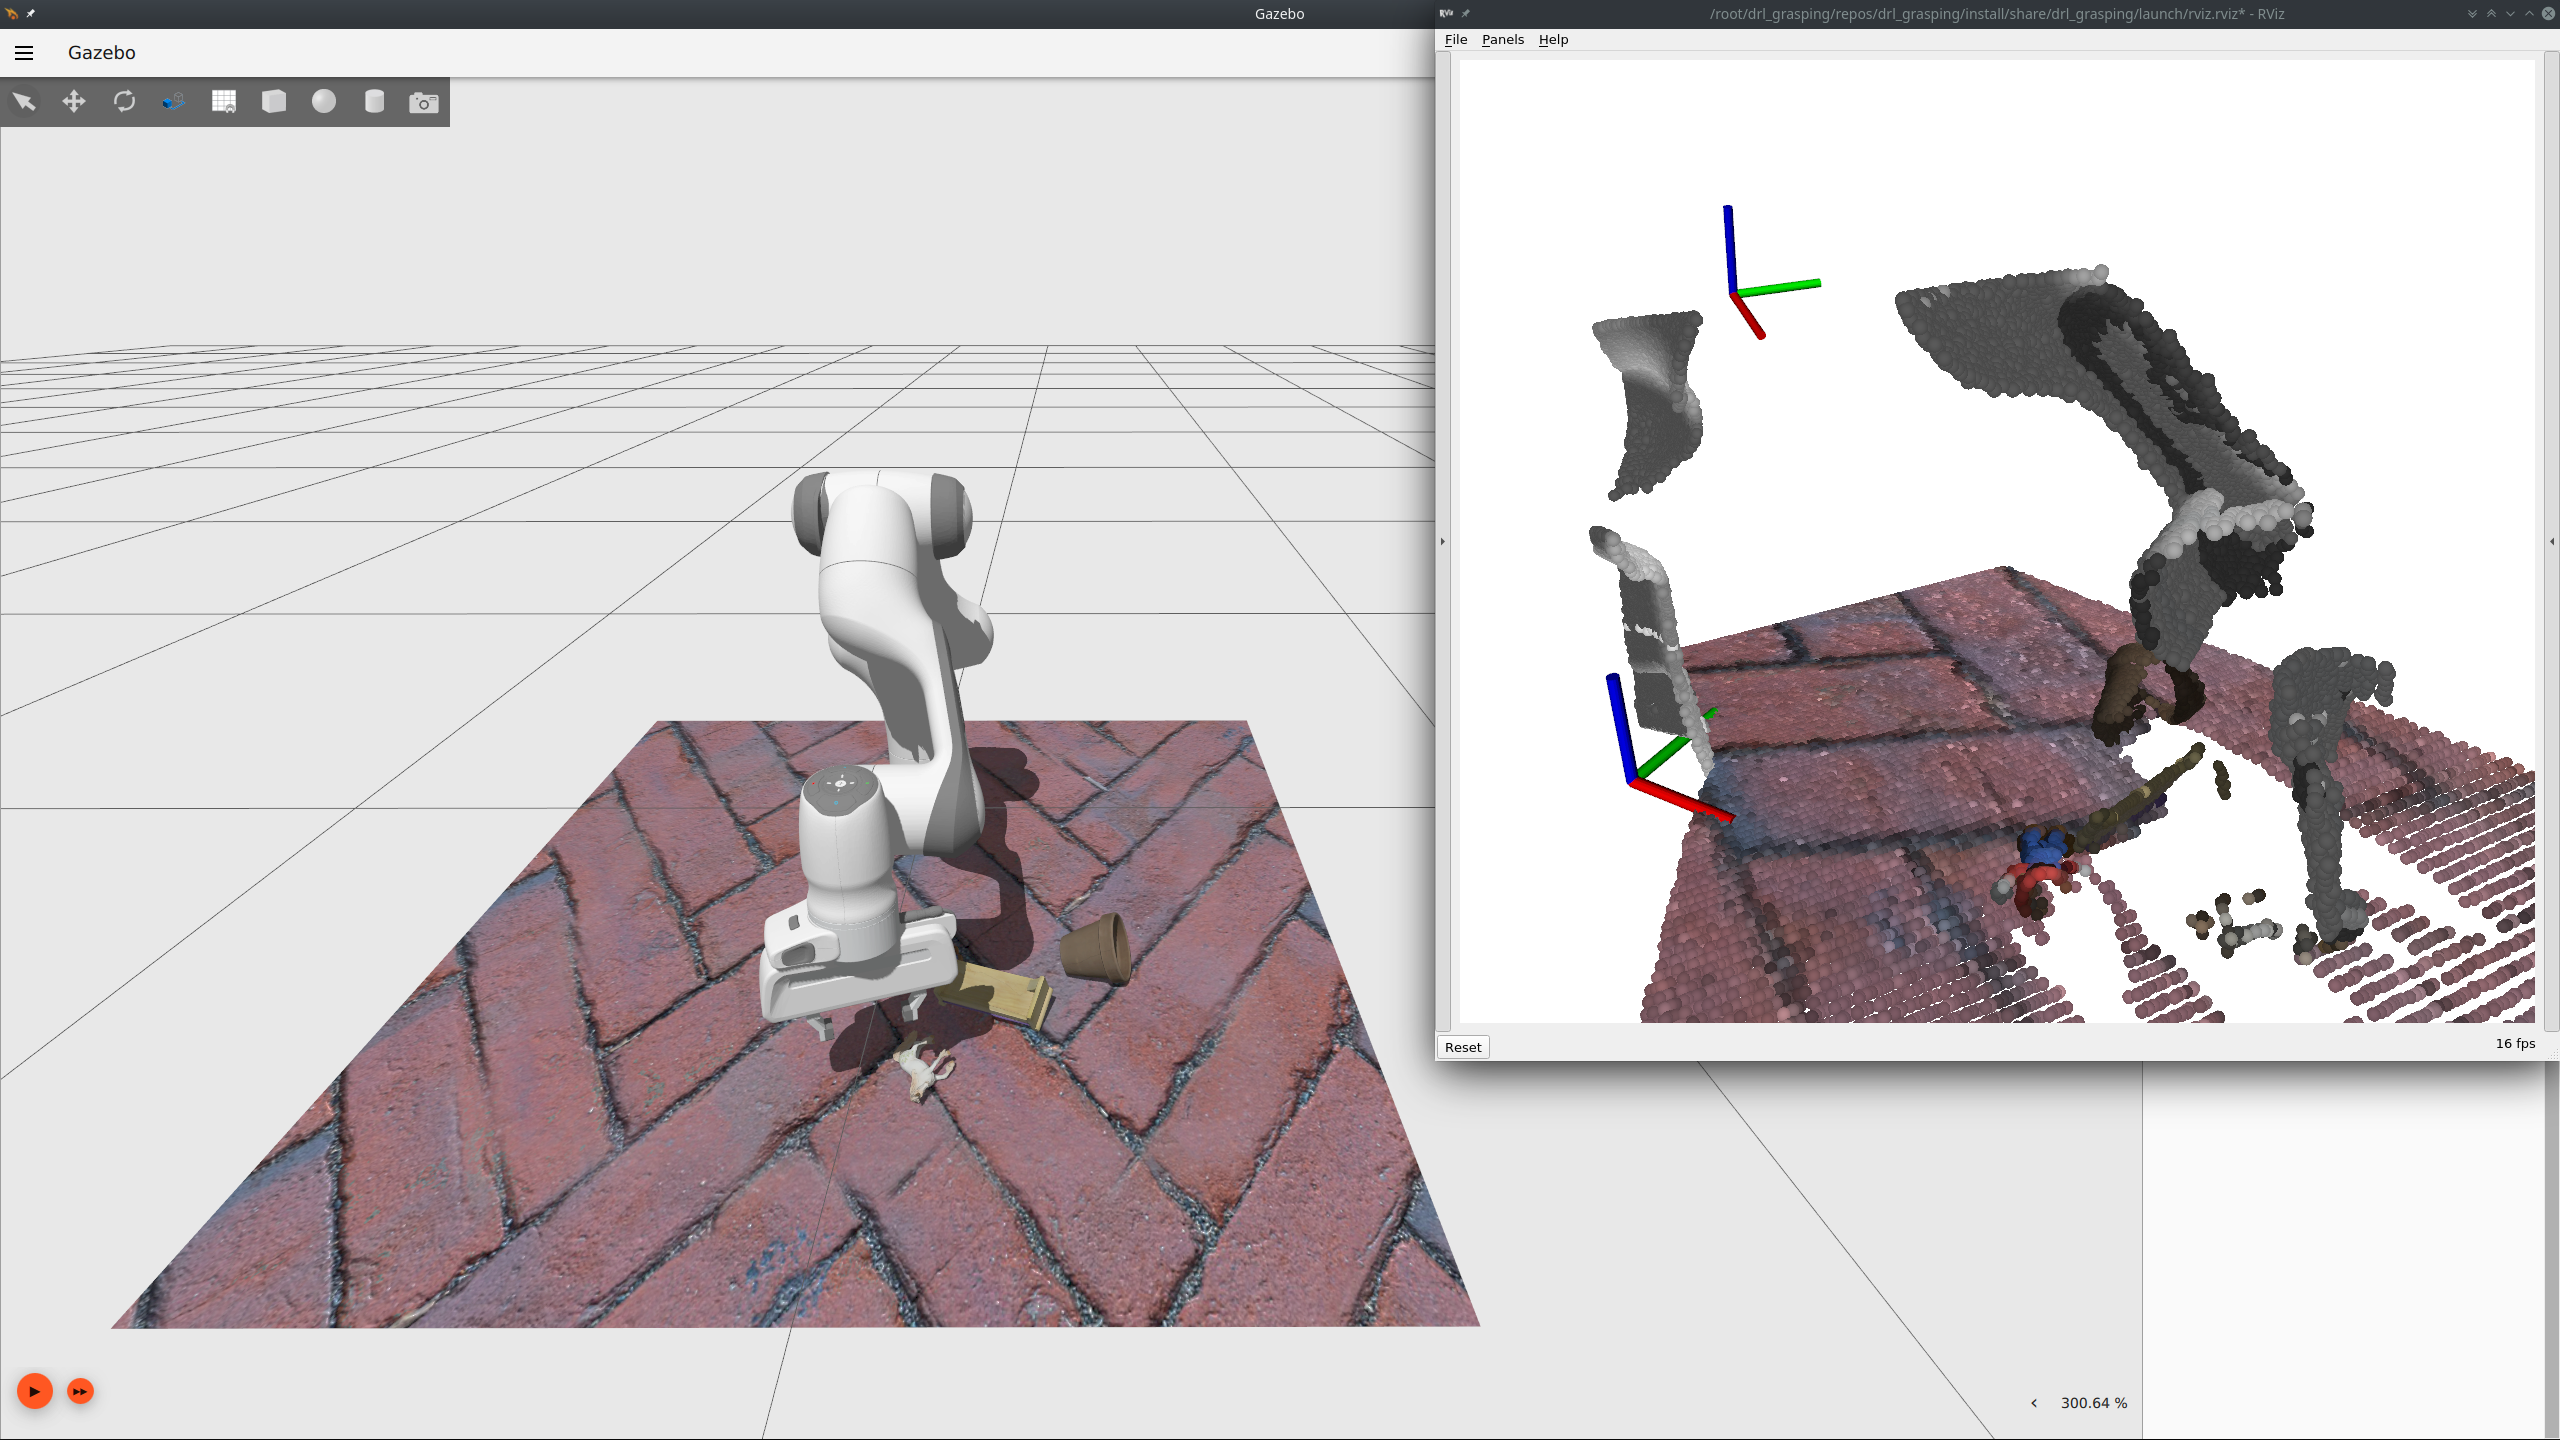
\includegraphics[height=3.8cm]{graphics/pre_trained_agent_example.png}
        \end{column}
    \end{columns}

    \begin{block}{Using Pre-Trained Agents}
        \begin{lstlisting}[language=bash,basicstyle=\tiny,stepnumber=1,numbersep=10pt,tabsize=4,showspaces=false,showstringspaces=false]
        drl_grasping/docker/run.bash andrejorsula/drl_grasping:latest ros2 run drl_grasping ex_enjoy_pretrained_agent.bash
        \end{lstlisting}
    \end{block}

    \vspace{0.5cm}

    \begin{block}{Training Your Own Agents}
        \begin{lstlisting}[language=bash,basicstyle=\tiny,stepnumber=1,numbersep=10pt,tabsize=4,showspaces=false,showstringspaces=false]
        drl_grasping/docker/run.bash andrejorsula/drl_grasping:latest ros2 run drl_grasping ex_train_agent.bash
        \end{lstlisting}
    \end{block}
\end{frame}
